\section{Attention Mechanism}
\label{sec:nlp_attention}
The attention mechanism mimics the retrieval of a value $v_i$ for a query $q$ based on a key $k_i$ in database.
$$attn(q, k, v) = \sum_i sim(q,k_i)\times v_i$$
\begin{figure}[h]
	\centering
	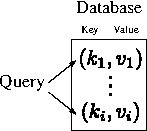
\includegraphics[scale=1.8]{./images/transformer/attention_database.pdf}
	\caption{The most similar key will be selected by measuring a \textbf{similarity} between a query and a key.}
\end{figure}

\begin{figure}[h]
	\centering
	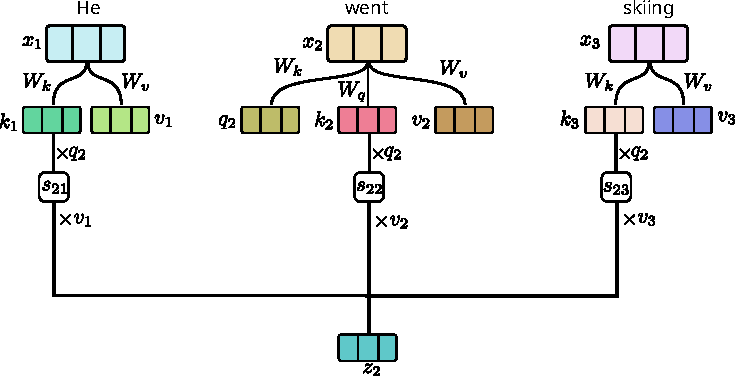
\includegraphics[scale=0.6]{./images/transformer/attention.pdf}
	\caption{The similarity $s_t$ is computed by a query and keys}
\end{figure}
There are several choices for a similarity function.
\begin{itemize}
	\item $q^Tk_i$: dot product.
	\item $\frac{q^Tk_i}{\sqrt{d}}$: scaled dot product $\to$ reduce the variance of the final attention weights. 
	\item $q^TWk_i$: general dot product.
	\item $w_q^Tq+ w_k^Tk_i$: additive similarity.
\end{itemize}
Finally, the \textbf{attention score} can be computed by using a softmax:
$$a_i = \frac{\exp(s_i)}{\sum_j \exp(s_j)}$$

\section{Transformer}
\label{sec:nlp_transformer}
% The encoder's inputs first flow through a self-attention layer – a layer that helps the encoder look at other words in the input sentence as it encodes a specific word. 


\subsection{Self-Attention}
$$attn(Q,K,V) = softmax\bigg(\frac{Q^TK}{\sqrt{d_k}}\bigg)V$$

Here, $Q, K, V\in \mathbb{R}^{N\times d}$, $QK^T$'s time complexity is $O(N^2d)$. This quadratic cost is massive for long input-sequences such as documents to be summarized or character-level inputs.


\subsection{Masked attention}
The masked attention is often referred to cross-attention. This is just a self-attention in decoder.
$$\textrm{MA}(Q,K,V) = softmax\bigg(\frac{Q^TK+M}{\sqrt{d_k}}\bigg)V,$$
where $M$ is a matrix of 0 and $-\infty$. Note that $-\infty$ will make $exp$ term to be zero.

\subsection{Skip Connection}
This is a regularization technique.

\subsection{Positional Embedding}

\begin{figure}[t]
	\centering
	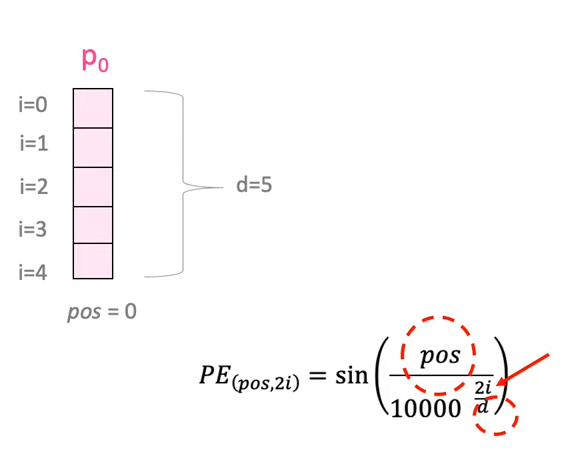
\includegraphics[scale=0.6]{./images/transformer/positional_1.png}
	\caption{Positional embedding.}
\end{figure}


\begin{lstlisting}[language=Python]
def position_encoding(seq_len: int, dim_model: int)->Tensor:
    pos = torch.arange(seq_len, dtype=torch.float).reshape(1, -1, 1)
    dim = torch.arange(dim_model, dtype=torch.float).reshape(1, 1, -1)
    phase = pos / (1e4 ** (dim // dim_model))
    return torch.where(dim.long() % 2 == 0, torch.sin(phase), torch.cos(phase))
\end{lstlisting}

\subsection{Encoder}

\subsection{Decoder}
The output of each step is fed to the bottom decoder in the next time step, and the decoders bubble up their decoding results just like the encoders did. And just like we did with the encoder inputs, we embed and add positional encoding to those decoder inputs to indicate the position of each word.

\begin{lstlisting}[language=Python]
def forward(self, tgt: Tensor, memory: Tensor) -> Tensor:
	seq_len, dimension = tgt.size(1), tgt.size(2)
	tgt += position_encoding(seq_len, dimension)
	for layer in self.layers:
		tgt = layer(tgt, memory)
	return torch.softmax(self.linear(tgt), dim=-1)
\end{lstlisting}





